%%%%%%%%%%%%%%%%%%%%%%%%%%%%%%%%%%%%%%%%%%%%%%%%%%%%%%%%%%%%%%%%%%%%%%%%%%%%%%%%%%%%%%%%%%%%%%%%%%%%%%%%%%%%%%%%%%%%%%%%%%%%%%%%%%%%%%%%%%%%%%%%%%%%%%%%%%%
% This is just an example/guide for you to refer to when submitting manuscripts to Frontiers, it is not mandatory to use Frontiers .cls files nor frontiers.tex  %
% This will only generate the Manuscript, the final article will be typeset by Frontiers after acceptance.   
%                                              %
%                                                                                                                                                         %
% When submitting your files, remember to upload this *tex file, the pdf generated with it, the *bib file (if bibliography is not within the *tex) and all the figures.
%%%%%%%%%%%%%%%%%%%%%%%%%%%%%%%%%%%%%%%%%%%%%%%%%%%%%%%%%%%%%%%%%%%%%%%%%%%%%%%%%%%%%%%%%%%%%%%%%%%%%%%%%%%%%%%%%%%%%%%%%%%%%%%%%%%%%%%%%%%%%%%%%%%%%%%%%%%

%%% Version 3.3 Generated 2016/11/10 %%%
%%% You will need to have the following packages installed: datetime, fmtcount, etoolbox, fcprefix, which are normally inlcuded in WinEdt. %%%
%%% In http://www.ctan.org/ you can find the packages and how to install them, if necessary. %%%
%%%  NB logo1.jpg is required in the path in order to correctly compile front page header %%%

\documentclass[utf8]{frontiersSCNS} % for Science, Engineering and Humanities and Social Sciences articles
%\documentclass[utf8]{frontiersHLTH} % for Health articles
%\documentclass[utf8]{frontiersFPHY} % for Physics and Applied Mathematics and Statistics articles

%\setcitestyle{square} % for Physics and Applied Mathematics and Statistics articles
\usepackage{url,hyperref,lineno,microtype,subcaption}
\usepackage[onehalfspacing]{setspace}
\usepackage{graphicx}
\usepackage{listings}
\usepackage{color}
\usepackage{lscape}
\usepackage[T1]{fontenc}

\definecolor{mygreen}{rgb}{0,0.6,0}
\definecolor{mygray}{rgb}{0.5,0.5,0.5}
\definecolor{mymauve}{rgb}{0.58,0,0.82}

\lstset{ %
  backgroundcolor=\color{white},   % choose the background color; you must add \usepackage{color} or \usepackage{xcolor}; should come as last argument
  basicstyle=\footnotesize,        % the size of the fonts that are used for the code
  breakatwhitespace=false,         % sets if automatic breaks should only happen at whitespace
  breaklines=true,                 % sets automatic line breaking
  captionpos=b,                    % sets the caption-position to bottom
  commentstyle=\color{mygreen},    % comment style
  deletekeywords={...},            % if you want to delete keywords from the given language
  escapeinside={\%*}{*)},          % if you want to add LaTeX within your code
  extendedchars=true,              % lets you use non-ASCII characters; for 8-bits encodings only, does not work with UTF-8
  frame=single,	                   % adds a frame around the code
  keepspaces=true,                 % keeps spaces in text, useful for keeping indentation of code (possibly needs columns=flexible)
  keywordstyle=\color{blue},       % keyword style
  language=Octave,                 % the language of the code
  morekeywords={*,...},            % if you want to add more keywords to the set
  numbers=left,                    % where to put the line-numbers; possible values are (none, left, right)
  numbersep=5pt,                   % how far the line-numbers are from the code
  numberstyle=\tiny\color{mygray}, % the style that is used for the line-numbers
  rulecolor=\color{black},         % if not set, the frame-color may be changed on line-breaks within not-black text (e.g. comments (green here))
  showspaces=false,                % show spaces everywhere adding particular underscores; it overrides 'showstringspaces'
  showstringspaces=false,          % underline spaces within strings only
  showtabs=false,                  % show tabs within strings adding particular underscores
  stepnumber=2,                    % the step between two line-numbers. If it's 1, each line will be numbered
  stringstyle=\color{mymauve},     % string literal style
  tabsize=2,	                   % sets default tabsize to 2 spaces
  title=\lstname                   % show the filename of files included with \lstinputlisting; also try caption instead of title
}



% Leave a blank line between paragraphs instead of using \\


\def\keyFont{\fontsize{8}{11}\helveticabold }
\def\firstAuthorLast{Sample {et~al.}} %use et al only if is more than 1 author
\def\Authors{First Author\,$^{1,*}$, Co-Author\,$^{2}$ and Co-Author\,$^{1,2}$}
% Affiliations should be keyed to the author's name with superscript numbers and be listed as follows: Laboratory, Institute, Department, Organization, City, State abbreviation (USA, Canada, Australia), and Country (without detailed address information such as city zip codes or street names).
% If one of the authors has a change of address, list the new address below the correspondence details using a superscript symbol and use the same symbol to indicate the author in the author list.
\def\Address{$^{1}$Laboratory X, Institute X, Department X, Organization X, City X , State XX (only USA, Canada and Australia), Country X \\
$^{2}$Laboratory X, Institute X, Department X, Organization X, City X , State XX (only USA, Canada and Australia), Country X  }
% The Corresponding Author should be marked with an asterisk
% Provide the exact contact address (this time including street name and city zip code) and email of the corresponding author
\def\corrAuthor{Corresponding Author}

\def\corrEmail{email@uni.edu}




\begin{document}
\onecolumn
\firstpage{1}

\title[NWB Query Engine]{NWB Query Engine: Efficient way to query neurophysiological data stored in Neurodata Without Borders format} 

\author[\firstAuthorLast ]{\Authors} %This field will be automatically populated
\address{} %This field will be automatically populated
\correspondance{} %This field will be automatically populated

\extraAuth{}% If there are more than 1 corresponding author, comment this line and uncomment the next one.
%\extraAuth{corresponding Author2 \\ Laboratory X2, Institute X2, Department X2, Organization X2, Street X2, City X2 , State XX2 (only USA, Canada and Australia), Zip Code2, X2 Country X2, email2@uni2.edu}


\maketitle


\begin{abstract}

%%% Leave the Abstract empty if your article does not require one, please see the Summary Table for full details.
\section{}
For full guidelines regarding your manuscript please refer to \href{http://www.frontiersin.org/about/AuthorGuidelines}{Author Guidelines}.

As a primary goal, the abstract should render the general significance and conceptual advance of the work clearly accessible to a broad readership. References should not be cited in the abstract. Leave the Abstract empty if your article does not require one, please see \href{http://www.frontiersin.org/about/AuthorGuidelines#SummaryTable}{Summary Table} for details according to article type. 


\tiny
 \keyFont{ \section{Keywords:} keyword, keyword, keyword, keyword, keyword, keyword, keyword, keyword} %All article types: you may provide up to 8 keywords; at least 5 are mandatory.
\end{abstract}

\section{Introduction}

Data coming from neurophysiological experiments are heterogeneous and organized in various data formats. A data format is usually given by hardware and software equipment defined by the specific device vendor. This format cannot be easily changed or reused in different devices. Nowadays with increasing computational performance and disk storages capacity researchers are more and more motivated to preserve not only experimental results but also original data used for performing analysis. A new modern concept calls such data as "Big Data" defined as  three Vs. (1) Volume defining big data as data from variety of sources , (2) Velocity defining big data as data coming from sensors by unprecedented speed, and	(3) Variety saying that data are in all types of formats. Moreover, neurophysiological data go even more behind this concept. Their are multimodal and dynamic because single experiment can involve several signal acquisition modalities. With increasing number of experiments the problem of non-standarised datasets stored in non-standarised formats makes  difficult an effective management and sharing. Researchers point out that data are even more important then papers describing results observed from the data. It is because if results are described in scientific papers without an access to the original datasets their validation or refinement over time is practically impossible. As a solution several attempts to provide a standardized way of data storing have appeared. These approaches vary from free-form data storages based on a simple data model providing only basic data structure \citep{10.3389/fninf.2011.00016} to rigid data formats often based on fixed schema technologies implemented in relational databases (e. g. SciDB \citep{Brown:2010:OSL:1807167.1807271}) requiring strictly defined set of attributes. Last approach includes data formats based on Semantic Web technologies that aims to machine readable data accessed via the Internet. 

Data formats based on a semantic web approach contains e.g.  NEMO \citep{DouFRFMT07} that describes classes of event-related brain potentials (ERP) and their properties. OBI \citep{citeulike:7291351} that is about scientific investigations, so OBI contains both general terms useful for any kind of experiment and also specific terms for specific kind of experiments. Every term has a unique identifier, standard metadata, and logical definitions that connect it to other terms in OBI, or OEN  \citep{10.3389/conf.fninf.2014.18.00044} that aims to cover devices and methods, and a  neurophysiological concepts derived from various data sources.

Lot of approaches are in preliminary implementation or do not provide satisfactory application interface. On the other hand lot of them are focused only on a specific purposes of a single laboratory. The most current and promising approach todays seems to be a Neurodata Without Borders (NWB) format its structure is based on conformity of various US universities and laboratories.

Once the first pilot version of the format and the API has been released \citep{teeters-neuron} questions on how to effectively query stored data raised. While relational databases based solutions are queried fairly easy by well-described SQL and data storages based on Semantic Web technologies are searchable solely by SPARQL \citep{prudhommeaux2008sparql} a satisfactory query engine for the NWB format does not exist yet.

As a solution the NWB Query engine that aims to provide an easy-to-use way to query dataset stored in the NWB format is presented.

The paper is organized as follows: Section \ref{materials_and_methods} describes state of the art in developing of data formats for neurophysiological experiments, existing frameworks for querying stored data and defines use-cases and specifications to the query engine. Then Section \ref{results} deals with the developed architectonic concept, describes implementation detail and a user perspective of the query engine. Last Section before Conclusion, Section \ref{Discussion} compares limitations of existing systems with the current one and points ideas for improvements.


\section{Material and Methods}
\label{materials_and_methods}

\subsection{Neurodata Without Borders Format}

Something about NWB specification, specification language, implementation in HDF5, NWB 1.0 vs. 2.0

\subsection{DataJoint}

\citep{Yatsenko031658}

\subsection{HDFql}

Maybe something about HDF5 API should be included as well.

\subsection{Query Engine High Level Specification}
\label{Query_engine_specification}
usecases

\subsection{Scope and Requirements}
\label{Scope_and_requirements}


\section{Results}
\label{results}

\subsection{Architecture}
\label{Architecture}

\subsection{Implementation}
\label{Implementation}

\begin{figure}
% Use the relevant command to insert your figure file.
% For example, with the graphicx package use
  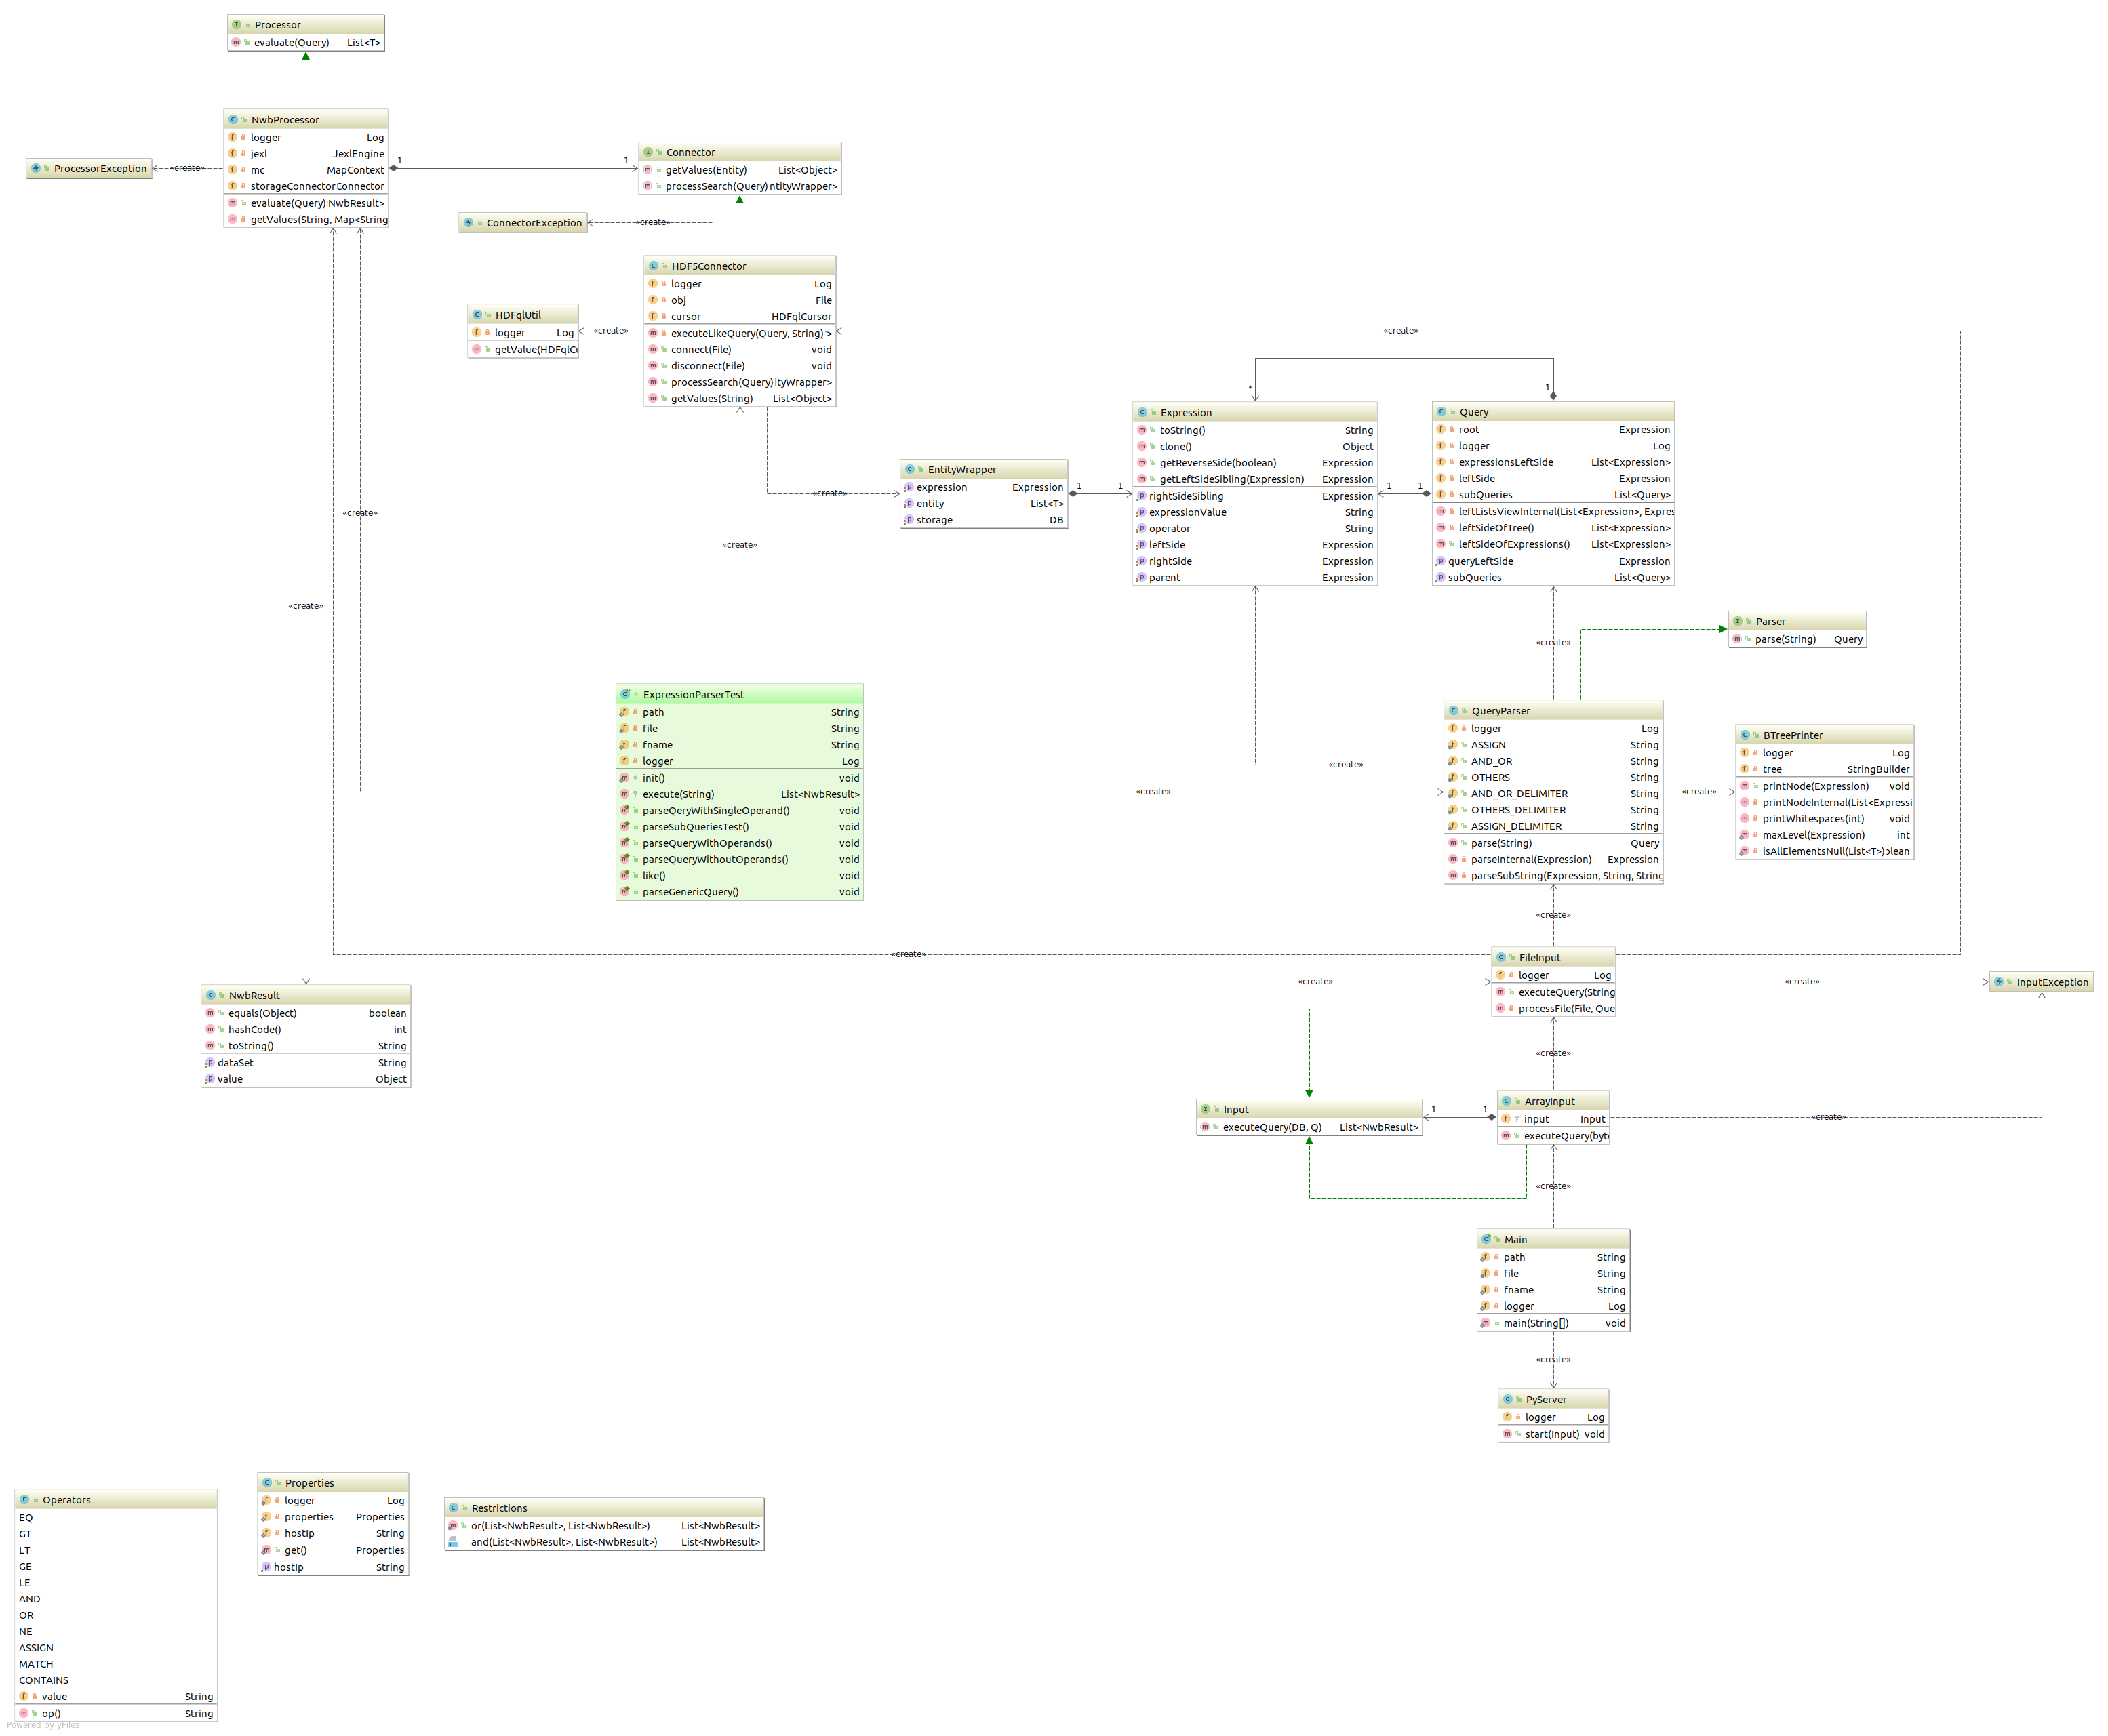
\includegraphics[width=17cm]{diagram}
% figure caption is below the figure
\caption{UML Diagram of the NWB Query Engine}
\label{fig:diagram}
\end{figure}

\subsubsection{Query Grammar}
\label{Query_Grammar}

\begin{itemize}  
\item gd = group|dataset
\item da = dataset|attribute
\item gd = (expression)
\item expression = expression | expression \& expression
\item expression = da < const | da <= const | da > const | da <= const | da LIKE const | gda
\end{itemize}

% For tables use
\begin{table}
% table caption is above the table
\caption{Query Examples}
\label{tab:query-examples}       % Give a unique label
% For LaTeX tables use

\begin{tabular}{ |p{7cm}|p{9cm}| }
\hline
	 \textbf{Query}                                  &       \textbf{Description} \\ \hline
	
	 analysis=(description LIKE whisker)  &  selects all datasets description from an analysis group which contains a whisker string  \\ \hline
	 processing=(electrode\_idx > 30)        &  selects all electrode\_idx datasets from a processing group which value > 30   \\ \hline
	 epochs=(start\_time > 200 \& stop\_time<400 \&\#124; stop\_time > 1600)  &  selects all epochs which start\_time > 200 and stop\_time < 400 or stop\_time > 1600 \\ \hline
	 epochs=(start\_time)                     &  selects all epochs with a start\_time dataset         \\ \hline
	 data=(unit LIKE unkno)  &  selects all datasets data with attributes containing a substring unkno \\ \hline
	 pole\_in/data=(unit LIKE unkno)  &  takes into account only data within a pole\_in group \\ \hline
	 analysis=(description LIKE whisker) \&\#124; epochs=(start\_time)   &  A combination of previous queries \\ \hline

\end{tabular}

\end{table}



\subsubsection{Operators}


\begin{itemize}
 \item and \&
 \item or  |
 \item equal ==
 \item assignment =
 \item brackets ()
 \item substrings in strings LIKE
\end{itemize}


\subsection{Python Gateway}
\label{Python_Gateway}

\begin{lstlisting}
 >>> from py4j.java_gateway import JavaGateway
 >>> from py4j.java_gateway import GatewayParameters
 >>> gateway = JavaGateway() # for localhost
 >>> gateway = JavaGateway(gateway_parameters=GatewayParameters(address='remote host ip')) # or for remote host
 >>> res = gateway.executeQuery("file or dir with nwb files", "query")
 >>> for x in res:
 ...     print (x)
\end{lstlisting}

\subsection{Web interface}
\label{web_interface}

\begin{figure}
% Use the relevant command to insert your figure file.
% For example, with the graphicx package use
  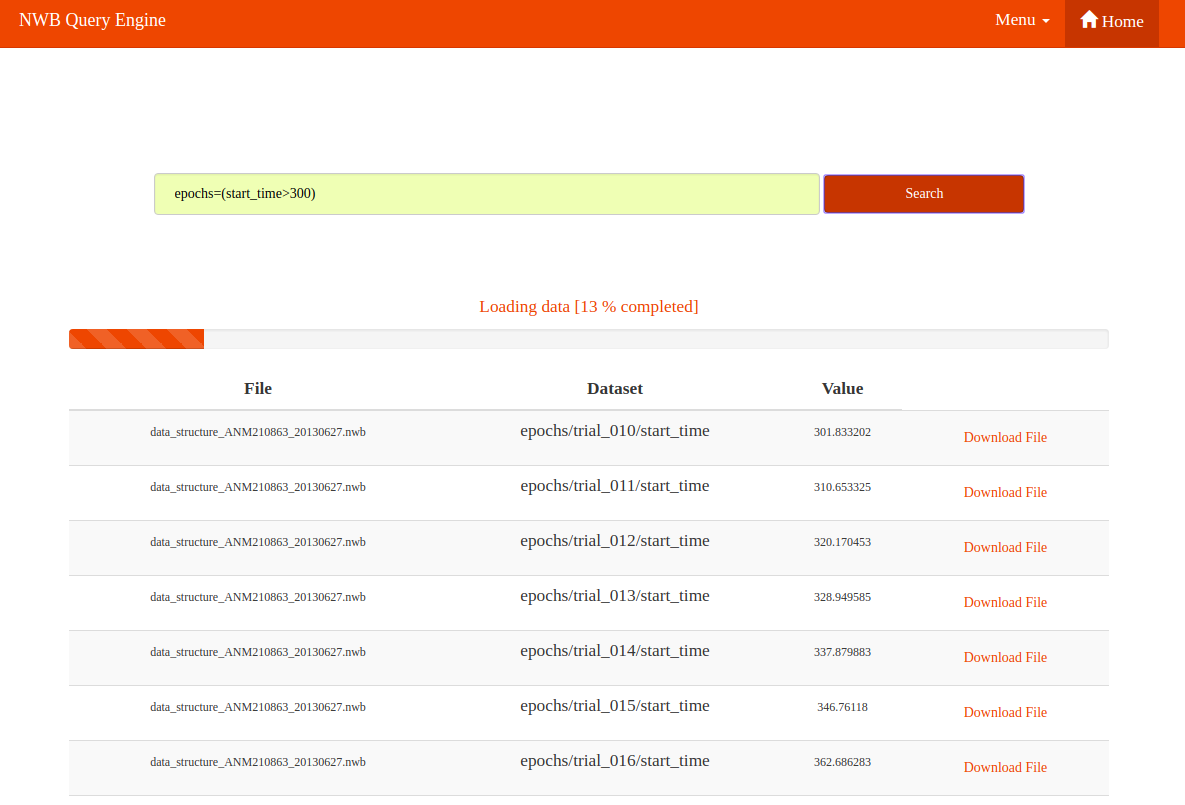
\includegraphics[width=17cm]{nwb-query-engine-web}
% figure caption is below the figure
\caption{NWB Query Engine Web Interface Preview}
\label{fig:diagram}
\end{figure}

\subsection{User Guide}
install steps etc.

Can be run as a library, as a command line application, as a python gateway or from the web

\section{Discussion}
\label{Discussion}

!todo! Comparrision of DataJoint, limitations of HDFql, why NWB Query Engine is such a good tool. What are its limits, how to solve them in the future?



\section*{Conflict of Interest Statement}
%All financial, commercial or other relationships that might be perceived by the academic community as representing a potential conflict of interest must be disclosed. If no such relationship exists, authors will be asked to confirm the following statement: 

The authors declare that the research was conducted in the absence of any commercial or financial relationships that could be construed as a potential conflict of interest.

\section*{Author Contributions}

The Author Contributions section is mandatory for all articles, including articles by sole authors. If an appropriate statement is not provided on submission, a standard one will be inserted during the production process. The Author Contributions statement must describe the contributions of individual authors referred to by their initials and, in doing so, all authors agree to be accountable for the content of the work. Please see  \href{http://home.frontiersin.org/about/author-guidelines#AuthorandContributors}{here} for full authorship criteria.

\section*{Funding}
Details of all funding sources should be provided, including grant numbers if applicable. Please ensure to add all necessary funding information, as after publication this is no longer possible.

\section*{Acknowledgments}
This is a short text to acknowledge the contributions of specific colleagues, institutions, or agencies that aided the efforts of the authors.

\section*{Supplemental Data}
 \href{http://home.frontiersin.org/about/author-guidelines#SupplementaryMaterial}{Supplementary Material} should be uploaded separately on submission, if there are Supplementary Figures, please include the caption in the same file as the figure. LaTeX Supplementary Material templates can be found in the Frontiers LaTeX folder 


\bibliographystyle{frontiersinSCNS_ENG_HUMS} % for Science, Engineering and Humanities and Social Sciences articles, for Humanities and Social Sciences articles please include page numbers in the in-text citations
%\bibliographystyle{frontiersinHLTH&FPHY} % for Health, Physics and Mathematics articles
\bibliography{nwb-query-engine}

%%% Make sure to upload the bib file along with the tex file and PDF
%%% Please see the test.bib file for some examples of references


\end{document}
